\documentclass[conference]{IEEEtran}
\usepackage{amsmath,amssymb,amsthm,bm,graphicx,booktabs,multirow,xcolor}
\usepackage[hidelinks]{hyperref}
\newtheorem{proposition}{Proposition}
\newtheorem{theorem}{Theorem}
\newtheorem{lemma}{Lemma}
\newtheorem{corollary}{Corollary}
\newcommand{\R}{\mathbb{R}}
\newcommand{\tr}{\operatorname{tr}}
\newcommand{\vect}{\operatorname{vec}}
\newcommand{\diag}{\operatorname{diag}}
\newcommand{\corank}{\operatorname{corank}}
\newcommand{\Log}{\operatorname{Log}}
\newcommand{\bx}{\bm{x}}
\newcommand{\bq}{\bm{q}}
\newcommand{\bth}{\bm{\theta}}
\newcommand{\bS}{\bm{\Sigma}}
\newcommand{\bR}{\bm{R}}
\newcommand{\bt}{\bm{t}}
\newcommand{\bH}{\bm{H}}
\newcommand{\bK}{\bm{K}}
\newcommand{\bW}{\bm{W}}

\newcommand{\bA}{\bm{A}}
\newcommand{\bI}{\bm{I}}
\newcommand{\bX}{\bm{X}}
\newcommand{\bM}{\bm{M}}
\newcommand{\bN}{\bm{N}}
\newcommand{\bQ}{\bm{Q}}
\newcommand{\bg}{\bm{g}}
\newcommand{\bh}{\bm{h}}
\newcommand{\bc}{\bm{c}}
\newcommand{\bG}{\bm{G}}
\newcommand{\bp}{\bm{p}}
\newcommand{\br}{\bm{r}}
\newcommand{\bb}{\bm{b}}
\newcommand{\be}{\bm{e}}
\newcommand{\bzero}{\bm{0}}
\newcommand{\Loss}{\mathcal{L}}
\newcommand{\ie}{i.e.,}
\newcommand{\eg}{e.g.,}
\newcommand{\etal}{et al.}

\title{Atomic Pose Layers: Selection-Aware Differentiation\\ for Quadratic Pose Estimation}
\author{\IEEEauthorblockN{Anonymous Authors}\\
\IEEEauthorblockA{Paper under review}}
\begin{document}
\maketitle

\begin{abstract}
We prove a face--stratum theorem for certifiable global geometric layers: a global pose layer admits a $C^1$ selection exactly when its optimal face is a single physical atom with a nonsingular KKT system ($k=1$, $m>0$, $\nu>0$). Value tightness and rank-one attainability are neither necessary nor sufficient: a loose lift can still have a $C^1$ map, and a tight rank-one lift can still expose two atoms. At a transversal tie no exact selection is continuous; smoothing must anneal its temperature with the margin; a fold pays $\nu^{-1/2}$. QPEP exposes the taxonomy: the $12\times12$ lift is tight with a unique atom and a two-to-one section resolved by $\det\bR=+1$; planar PnP has two equal-cost atoms; the noiseless quaternion gap is zero. We instantiate this as Atomic Pose Layers (a face/branch certificate, a three-state API, and a certificate-gated softmin). On a minimal 3-point PnP benchmark, cue-conditioned selection reaches $80.8\%$ versus $64.4\%$ for cue-initialized local solving (oracle $89.6\%$); a same-start ablation attributes the gain to selection, and a P3P+cue baseline reaches $86.6\%$, locating the gap in the QPEP candidate set.\end{abstract}

\section{Introduction}
Quadratic pose estimation (QPEP) unifies PnP, hand--eye calibration, point-to-plane registration, and multi-robot relative pose as a quaternion-constrained polynomial problem \cite{wu2022qpep}. A differentiable QPEP layer is an attractive geometric front end for robot learning: a perception network predicts measurements, the layer returns a pose, and a controller or world model consumes it. The forward global solver, however, does not return a function: it returns one of several stationary branches. Existing differentiable optimization layers either differentiate a local solver \cite{amos2017optnet,pineda2022theseus,chen2020bpnp} or assume that a Shor relaxation is tight and rank-one \cite{holmes2025sdpr}. Neither assumption holds at a global switch.

The central question is therefore not how to differentiate a solver, but \emph{what object carries a derivative}: the \emph{optimal face}, not the optimal value.

First, the rotation-matrix lift is routinely misdiagnosed. For generic PnP, the $12\times12$ lift is tight and returns a unique rank-one $\bX^\star=\bx\bx^\top$; the sign of $\bx$ is a two-to-one section, resolved by $\det\bR=+1$. The reported ``$1.73$ orthogonality error and $\det R=0$'' is the last row of a rank-two barycenter of the $13\times13$ homogenization ($R=0$), not a tightness failure.

Second, planar PnP has an exact flip: the true pose and its flip have identical cost. Here the face is genuinely multi-atomic (two rank-one atoms); no image-only gradient can choose between them, and a prior or task cue is required.

Third, the quaternion moment gap is vacuous on noiseless data: the cost is a sum of squares, so both the minimum and the moment bound are zero. The gap carries no identifiability information; the face does, since every optimal $\bM$ satisfies $\bW\bM=0$ and $\mathrm{rank}(\bM)\le\dim\ker\bW$. A ``gap-aware'' layer that treats $\Delta\le\tau$ as certified is therefore not a certificate.

Our core result is a \emph{face--stratum theorem} (Theorem~\ref{thm:face-stratum}): a $C^1$ selection exists exactly when the optimal face is a single physical atom with a nondegenerate KKT system. Outside it, a tie/fold dichotomy (Theorem~\ref{thm:nfl}) gives no exact continuous selection at a transversal tie; smoothing must anneal with the margin (Corollary~\ref{cor:smoothing}); a fold pays $\nu^{-1/2}$. We instantiate the theorem as Atomic Pose Layers and validate the selection layer on a minimal 3-point PnP benchmark.

The contributions are:
\begin{itemize}
\item \textbf{Face--stratum theorem (core).} Under A1--A5, a $C^1$ selection exists iff $k=1$, $m>0$, $\nu>0$, with derivative $-\bK^{-1}\bN$; the gate is the face, not the gap or the rank.
\item \textbf{Value--face separation, both directions.} On noiseless QPEP $\Delta=0$ and $\bW\bM=0$, so $\mathrm{rank}(\bM)\le\dim\ker\bW$. Neither $\Delta=0$ nor rank-one attainability implies a unique atom (planar flip; R-form section), and neither is necessary (a loose lift with a unique atom is still $C^1$).
\item \textbf{Tie/fold dichotomy.} At a transversal tie no selection that is exact off the tie is continuous at it; the set-valued solution map is Hausdorff-continuous but not single-valued, while the value is continuous. Smoothing keeps an $e^{-m/\tau}$ wrong-branch mass, so its temperature must vanish with the margin; at a fold the branch derivative diverges as $\nu^{-1/2}$.
\item \textbf{Atomic Pose Layers.} A face/branch certificate, a three-state API (CERTIFIED/AMBIGUOUS/VALUE-ONLY), and a certificate-gated Gibbs/softmin. On the minimal 3-point PnP benchmark, cue-conditioned selection reaches $80.8\%$ versus $64.4\%$ for cue-initialized local solving; a same-start ablation shows the gain is selection, not extra starts, and a P3P multi-solution baseline locates the remaining recall gap.
\end{itemize}

\section{Related Work}
\paragraph{Global pose estimation.} QPEP \cite{wu2022qpep} derives the quaternion cost, enumerates all KKT roots with Gr\"obner bases, and estimates covariance via a semidefinite program; sQPEP \cite{xue2025sqpep} extends it to scale. These works provide a forward global solver but no derivative or branch certificate.

\paragraph{Certifiable and differentiable layers.} SDPRLayers \cite{holmes2025sdpr} proves a correct Jacobian for a tight Shor QCQP under rank one and $\corank\bH=1$; the non-tight fallback has no guarantee, and multiple global optima are explicitly not handled. The Cayley-map approach \cite{barfoot2025cayley} removes reflections by parameterization and extends to trajectories; C2P \cite{tirado2024c2p} handles cheirality explicitly for relative pose. OptNet \cite{amos2017optnet}, Theseus \cite{pineda2022theseus}, and black-box QP differentiation \cite{magoon2025dqp} differentiate convex or local problems; BPnP \cite{chen2020bpnp} is the local PnP baseline whose failure mode motivates our face analysis. Entropic smoothing, perturbed optimizers \cite{berthet2020perturbed}, and black-box differentiation \cite{vlastelica2020blackbox} are the standard escapes from a non-differentiable argmin. We call the resulting contract \emph{Face-Certified Differentiation} (FCD) and instantiate it as Atomic Pose Layers; unlike a smoother, FCD refuses to return a pose when the face is not a single physical atom.

\paragraph{Nonsmooth sensitivity.} The value function of a parametric program is locally Lipschitz and its Clarke subdifferential is the convex hull of active branch gradients; the solution map is not locally Lipschitz at a tie and has no Clarke Jacobian. We use this classical distinction (see \cite{clarke1983,luo1996,jongen2004}) not as a contribution but as the reason a \emph{face} contract is needed.

\section{Face--Stratum Theory and QPEP}
\subsection{Quaternion cost and exact elimination}
Let $\bq\in\R^4$ be a unit quaternion and $\bR(\bq)$ its rotation. For correspondence $i$, let $\bp_i\in\R^3$ and $(u_i,v_i)$ be normalized image coordinates. The algebraic residual is
\begin{equation}
\br_i(\bq,\bt)=
\begin{bmatrix}
u_i\be_3^\top(\bR\bp_i+\bt)-\be_1^\top(\bR\bp_i+\bt)\\
v_i\be_3^\top(\bR\bp_i+\bt)-\be_2^\top(\bR\bp_i+\bt)
\end{bmatrix}.
\end{equation}
With $J=\sum_i\|\br_i\|^2$, fixed $\bq$ gives $\br_i=\bA_i\bt+\bb_i(\bq)$ with $\bA_i$ constant and $\bb_i$ quadratic. Hence
\begin{align}
\bG&=\sum_i\bA_i^\top\bA_i,\quad \bh(\bq)=\sum_i\bA_i^\top\bb_i(\bq),\\
J(\bq)&=\bc(\bq)-\bh(\bq)^\top\bG^{-1}\bh(\bq),\quad \bt(\bq)=-\bG^{-1}\bh(\bq),
\end{align}
a quartic in $\bq$ on the unit sphere. The KKT system is
\begin{equation}
\nabla J(\bq)-\lambda\bq=\bzero,\qquad \bq^\top\bq=1,
\label{eq:kkt}
\end{equation}
with KKT matrix
\begin{equation}
\bK=\begin{bmatrix}\nabla^2J-\lambda\bI&-\bq\\2\bq^\top&0\end{bmatrix}.
\label{eq:K}
\end{equation}
The gauge $\bq\sim-\bq$ leaves $\bR$ invariant; we differentiate the physical output.

\subsection{Tightness taxonomy}
Let $F(\bth)$ be the optimal face of a lifted SDP, $\bH$ its dual certificate, and $k$ the number of active branches. We distinguish:
\begin{enumerate}
\item \textbf{value-tight}: the SDP value equals the primal minimum;
\item \textbf{rank-one-attainable}: $F$ contains at least one rank-one atom $xx^\top$;
\item \textbf{rank-one-returned}: the solver returns such an atom;
\item \textbf{unique}: $F$ is a single rank-one atom.
\end{enumerate}
Only the last class supports a single pose and a single derivative. The taxonomy separates three failure modes that the literature often conflates: a loose relaxation, a tight relaxation with a non-unique face, and a solver that returns an interior point of a non-unique face.

\subsection{R-form: one atom, a two-to-one section}
With $\bx=[\vect(\bR);\bt]\in\R^{12}$, the algebraic cost is $J(\bx)=\bx^\top\bQ\bx$ and the orthogonality constraints are $\bR^\top\bR=\bI$. The $12\times12$ Shor relaxation is
\begin{equation}
\min_{\bX\succeq0}\langle\bQ,\bX\rangle
\ \text{s.t.}\ \langle\bA_{ab},\bX\rangle=\delta_{ab}.
\label{eq:rform}
\end{equation}
For generic PnP, $\mathrm{rank}(\bX^\star)=1$, $\|\bR^\top\bR-\bI\|_F\approx10^{-11}$, $\det\bR=\pm1$. Since $\bX^\star=\bx\bx^\top$, the map $\bx\mapsto\bX$ is two-to-one: the face is a \emph{single} rank-one atom, and the sign is a section ambiguity, not a multi-atom face; $\det\bR=+1$ selects the proper pose, so generic PnP needs no cue. The $13\times13$ homogenization's last-row section yields $\bR=0$, hence the artifact $\|\bR^\top\bR-\bI\|_F=\sqrt3$, $\det\bR=0$; a correct $12$-block section recovers $\pm\bR_{\mathrm{gt}}$.

\subsection{q-form: the noiseless gap is vacuous}
Write $J(\bq)=m(\bq)^\top\bW m(\bq)$ with $m$ the degree-$\le2$ monomial vector and $\bW\succeq0$ the Gram matrix of the residual coefficients. On noiseless data $J(\bq_{\mathrm{gt}})=0$, so the moment lower bound is $0$; the value gap is zero for \emph{every} instance and carries no identifiability information. Any optimal moment matrix $\bM$ satisfies $\langle\bW,\bM\rangle=0$ with both PSD, hence $\bW\bM=0$ and $\mathrm{range}(\bM)\subseteq\ker\bW$. Consequently
\begin{equation}
\mathrm{rank}(\bM)\le\dim\ker\bW,
\label{eq:ker}
\end{equation}
and the nullity of $\bW$, not the gap, is the identifiability measure. On generic PnP we observe $\dim\ker\bW=6$--$7$ and numerical $\mathrm{rank}(\bM)\le\dim\ker\bW$ at a consistent tolerance (Table~\ref{tab:diag}); the solver returns a non-extreme point of the face. The rank is not a certificate of non-existence of a rank-one optimum.

\begin{theorem}[Value--face separation]
\label{thm:value-face}
On noiseless QPEP, $J(\bq_{\mathrm{gt}})=0$, the moment lower bound is $0$, and the value gap vanishes for every instance. Every optimal moment matrix satisfies $\bW\bM=0$, hence $\mathrm{range}(\bM)\subseteq\ker\bW$ and $\mathrm{rank}(\bM)\le\dim\ker\bW$. Moreover:
(a) \emph{[not sufficient]} $\Delta=0$ and rank-one attainability do not certify a unique differentiable layer: planar PnP has two equal-cost rank-one atoms, and the R-form's unique $\bX$ still leaves the two-to-one section $\bx\mapsto\bx\bx^\top$, resolved only by the physicality constraint $\det\bR=+1$;
(b) \emph{[not necessary]} a unique physical atom with a $C^1$ solution map can coexist with a loose lift (positive gap) and with a returned $\bM$ of rank $6$--$7$.
Hence neither $\Delta$ nor the rank of the returned $\bM$ certifies a differentiable physical layer.
\end{theorem}
\begin{proof}
$J(\bq)=\bm{m}(\bq)^\top\bW\bm{m}(\bq)$ is a sum of squares; $J(\bq_{\mathrm{gt}})=0$ gives lower bound $0$ and gap $0$. If $\bM\succeq0$ is optimal, $\langle\bW,\bM\rangle=0$ with $\bW\succeq0$ implies $\bW\bM=0$; hence $\mathrm{range}(\bM)\subseteq\ker\bW$.
(a) On the planar instance, the true pose and its flip are two distinct rank-one atoms $\bX_1\ne\bX_2$ with equal cost and gap $0$ (Section~\ref{sec:planar}). For the R-form, a unique $\bX=\bx\bx^\top$ is compatible with both $\bx$ and $-\bx$; only the physicality constraint $\det\bR=+1$ resolves the section.
(b) Table~\ref{tab:diag} reports noisy q-form instances with positive gaps and $\mathrm{rank}(\bM)=6$--$7$; the physical minimizer is isolated up to the gauge $\bq\sim-\bq$, and differentiability follows from Theorem~\ref{thm:face-stratum}(i).
\end{proof}

\subsection{Face--branch duality}
\begin{lemma}[Face--branch duality]
\label{lem:face-branch}
Assume strong duality and attainability, an exact relaxation, strict complementarity $\ker\bH=\mathrm{range}(\bX)$, isolated global minima, and face realizability. Then
\begin{multline}
\mathrm{range}(\bX)=\mathrm{span}\{\bq_j\bq_j^\top: j\in J(\bth)\},\\
\corank\bH=\dim\mathrm{span}\{\bq_j\}=k
\label{eq:duality}
\end{multline}
generically. In particular $\corank\bH=1$ iff $k=1$; for $k=2$ the face is the segment $\bX=\omega\bq_1\bq_1^\top+(1-\omega)\bq_2\bq_2^\top$ and the same certificate certifies both branches.
\end{lemma}
The proof is the standard face argument: $\bH\bX=0$ with both PSD gives $\mathrm{range}(\bX)\subseteq\ker\bH$; strict complementarity gives equality; exactness and feasibility put each $\bq_j\bq_j^\top$ in the face; realizability gives the reverse inclusion; dimension counting gives the corank.

\begin{theorem}[Face--stratum and the tie dichotomy]
\label{thm:face-stratum}
Assume (A1) strong duality and attainability, (A2) exactness of the lift, (A3) strict complementarity, (A4) isolated physical global minima with SOSC/ACQ, and (A5) face realizability. Let $k$ be the number of distinct physical global atoms modulo the gauge $\bq\sim-\bq$, $m>0$ the tie margin, and $\nu=\sigma_{\min}(\bK)/\sigma_{\max}(\bK)>0$. Then:
(i) if $k=1$ and $\nu>0$, the global solution map is $C^1$ and $\frac{d\bq}{d\bth}=-\bK^{-1}\bN$;
(ii) if $k\ge2$ and the tie at $\bth^\star$ is \emph{transversal}---$\bq_1(\bth^\star)\ne\bq_2(\bth^\star)$ are both global, and for some $\epsilon>0$ exactly one of them is the unique global minimizer on each side of $\bth^\star$, with the winner swapping---then no selection that equals the global minimizer for all $\bth\ne\bth^\star$ is continuous at $\bth^\star$. In particular no exact continuous Lipschitz selection exists;
(iii) if $k=1$ and $\nu=0$ (fold), the map is not $C^1$ and the branch derivative diverges as $\nu^{-1/2}$.
\end{theorem}
\begin{proof}
(i) By Lemma~\ref{lem:face-branch}, $k=1$ gives $\bX=\bq\bq^\top$; the KKT system $F(\bq,\lambda;\bth)=0$ has nonsingular Jacobian $\bK$ when $\nu>0$; the implicit function theorem gives $C^1$ and the derivative. (ii) Let $s$ be exact off the tie. For $\bth<\bth^\star$, $s(\bth)=\bq_1(\bth)$ and for $\bth>\bth^\star$, $s(\bth)=\bq_2(\bth)$ (after relabeling). If $s$ is continuous at $\bth^\star$, then $\bq_1(\bth^\star)=\lim_{\bth\uparrow\bth^\star}s(\bth)=\lim_{\bth\downarrow\bth^\star}s(\bth)=\bq_2(\bth^\star)$, contradicting $\bq_1(\bth^\star)\ne\bq_2(\bth^\star)$. The set-valued solution map is Hausdorff-continuous at $\bth^\star$ (both branches converge to their limits and both are included at $\bth^\star$), and the value $\min(J_1,J_2)$ is continuous; what fails is single-valuedness, not continuity of the set map. (iii) At a fold $\bK$ is singular; the saddle-node normal form gives $|\bq_+-\bq_-|\sim\sqrt{\nu}$ and $|d\bq/d\bth|\sim\nu^{-1/2}$; no $C^1$ map. The gap/rank statements are Theorem~\ref{thm:value-face}.
\end{proof}

\begin{corollary}[Smoothing must anneal with the margin]
\label{cor:smoothing}
For $\bth$ with margin $m(\bth)>0$, let $L_\tau=-\tau\log\sum_j e^{-J_j/\tau}$ and $w_j\propto e^{-J_j/\tau}$. Then
\begin{equation}
0\le L_\tau-\min_j J_j\le \tau\log k,\qquad
\sum_{j\ne j^\star}w_j\le (k-1)e^{-m(\bth)/\tau}.
\label{eq:smooth}
\end{equation}
To keep the total wrong-branch mass below $\delta$, one needs $\tau\le m(\bth)/\log((k-1)/\delta)$. Hence a fixed temperature is inexact at a tie, and its gradient retains an $e^{-m/\tau}$ bias.
\end{corollary}
\begin{proof}
The first bound is Jensen's inequality and the log-sum-exp bound. Since $J_j-J_{j^\star}\ge m$, $\sum_{j\ne j^\star}w_j\le(k-1)e^{-m/\tau}/(1+(k-1)e^{-m/\tau})\le(k-1)e^{-m/\tau}$; solving for $\tau$ gives the annealing rule.
\end{proof}


\section{Atomic Face Certification and Differentiation}
\subsection{Branch--margin derivative certificate}
Define the tie margin and fold margin
\begin{equation}
m(\bth)=\min_{j\notin J(\bth)}(J_j-J_{j^\star}),\qquad
\nu(\bth)=\frac{\sigma_{\min}(\bK)}{\sigma_{\max}(\bK)}.
\label{eq:margins}
\end{equation}
\begin{corollary}[Branch--margin derivative]
\label{cor:branch-margin}
On the open stratum
$\mathcal{U}=\{k=1,\ m>0,\ \nu>0,\ \mathrm{SOSC},\ \mathrm{ACQ}\}$,
the global solution map is $C^1$ and equals the selected branch, with
\begin{equation}
\frac{d\bq}{d\bth}=-\bK^{-1}\bN,
\label{eq:ift}
\end{equation}
where $\bN$ is the derivative of the KKT residual. The statement uses no value gap, rank, or tightness assumption.
\end{corollary}
Corollary~\ref{cor:branch-margin} is Theorem~\ref{thm:face-stratum}(i) with the margin definitions; a value certificate is neither necessary nor sufficient for a derivative certificate. The correct gate is the pair $(m,\nu)$ plus the face multiplicity $k$.

\subsection{Switch dichotomy and folds}
\begin{theorem}[No-free-lunch at a switch]
\label{thm:nfl}
Under the hypotheses of Theorem~\ref{thm:face-stratum}(ii), every selection is either inexact for some $\bth\ne\bth^\star$ or discontinuous at $\bth^\star$. A selection that is continuous at $\bth^\star$ and agrees with the global minimizer on one side must disagree with it on the other; if it stays within $\delta$ of the exact argmin on both sides, then $\delta\ge\|\bq_1-\bq_2\|/2$. The value $V(\bth)=\min_jJ_j(\bth)$ is locally Lipschitz, with Clarke subdifferential $[\min(J_1',J_2'),\max(J_1',J_2')]$ at $\bth^\star$; the solution map is Hausdorff-continuous but not single-valued. At a fold $\nu\to0$, the branch derivative diverges as $\nu^{-1/2}$.
\end{theorem}
\begin{proof}
The first sentence is Theorem~\ref{thm:face-stratum}(ii). If a continuous selection agrees with $\bq_1$ on one side and $\bq_2$ on the other, its distance to the exact argmin is at least $\|\bq_1-\bq_2\|/2$ somewhere; the bound follows. The Clarke formula is the max rule for two $C^1$ branches; the fold statement is Theorem~\ref{thm:face-stratum}(iii).
\end{proof}
Smoothing therefore does not remove the price: it moves it into a temperature that must vanish with $m(\bth)$ (Corollary~\ref{cor:smoothing}). Unrolling differentiates a different map. This is a no-free-lunch statement for continuous differentiable global layers, not an implementation detail.

\paragraph{Machine-checked 1-D core.} The 1-D tie bound (no continuous selection of the global minimizer of $(x^2-1)^2+\theta x$ can take either value $\pm1$ at $\theta=0$) and the rank component of Theorem~\ref{thm:value-face} ($\bW\bM=0\Rightarrow\mathrm{range}(\bM)\subseteq\ker\bW$, $\mathrm{rank}(\bM)\le\dim\ker\bW$) are machine-checked in Lean~4 (toolchain \texttt{v4.34.0-rc2}, Mathlib commit \texttt{85e3a25}) in \texttt{lean/FaceStratum/Tie.lean} and \texttt{lean/FaceStratum/ValueFace.lean}; \texttt{lake build} completed successfully (8766 jobs). The Lean 1-D theorem is the special case of an exact tie at every $\theta$ (the global minimizer is $\pm1$ for all $\theta$); the exact-off-tie and Lipschitz clauses of Theorem~\ref{thm:face-stratum}(ii) are proved on paper, not in Lean. The PSD step $\tr(\bW\bM)=0\Rightarrow\bW\bM=0$ is proved here via the spectral theorem; the general face--stratum and SDP/KKT/IFT formalization remain future work.

\subsection{Three-state API}
Given a lifted SDP and a numerical dual $\bH$:
\begin{enumerate}
\item \textbf{VALUE-ONLY}: if $\bH$ is not PSD to tolerance or $\bH\bX\not\approx0$, return only the bound; never a pose or derivative.
\item \textbf{CERTIFIED}: if $\mathrm{rank}(\bX)=1$, the atom is physical (rotation, positive depth), and $m>0,\nu>0$, return the pose, the KKT derivative \eqref{eq:ift}, and $(m,\nu)$.
\item \textbf{AMBIGUOUS}: if the face has multiple physical atoms, return the branch/atom set, the Jacobian set, the switch margin, and a branch-mixture covariance; do not collapse to one pose.
\end{enumerate}
The API is the main practical consequence: a geometric layer can say ``I do not know which branch'' instead of silently returning a wrong gradient. The states are a contract: in this paper the SCS dual is numerical (Section~\ref{sec:exp}), so a CERTIFIED state requires an explicit PSD/tolerance check and is not claimed from the diagnostic alone.

\paragraph{Atomic selection-aware differentiation (ASAD).} For an ambiguous face, one may expose a temperature-annealed mixture of branch derivatives, $L_\tau=\sum_jw_jL_j$ with $w_j\propto e^{-J_j/\tau}$. Its gradient has the branch term and the selection term
\begin{equation}
\nabla L_\tau=\sum_jw_j\nabla L_j-\frac{1}{\tau}\sum_jw_j(L_j-\bar L)\nabla J_j.
\label{eq:selection}
\end{equation}
The selection term is the mollified jump of the discontinuous hard loss; it is a decision under a prior or task cue, not a certificate. Pure Clarke (uniform weights, no selection term) is legal but not unique; the selection term is what can train a cue-conditioned measurement map. By Corollary~\ref{cor:smoothing}, a fixed temperature keeps a wrong-branch mass of order $e^{-m/\tau}$, so $\tau$ must anneal with the margin. On a fixed-hypothesis model whose branch losses are constant, so the local and hard-global branch gradients are identically zero, a 200-step descent leaves the hard/local loss at $4.00$; the selection-aware descent reaches $0.00$. This isolates the selection term from the branch derivative.

\paragraph{Covariance.} On the ambiguous face we return a mixture on $\mathrm{SO}(3)$, not in raw quaternion coordinates:
\begin{equation}
\bS_{\rm mix}=\sum_jw_j\left(\bS_j+\Log(\bar\bR^\top\bR_j)\Log(\bar\bR^\top\bR_j)^\top\right),
\label{eq:cov}
\end{equation}
with $\bar\bR$ the weighted Fr\'echet mean, $w_j$ Laplace-evidence weights, and an abstention mass when the face is not certified. Equation~\eqref{eq:cov} removes the spurious variance that a raw $\bq/\bR$ mixture would create for the gauge pair.

\begin{figure*}[!t]
\centering
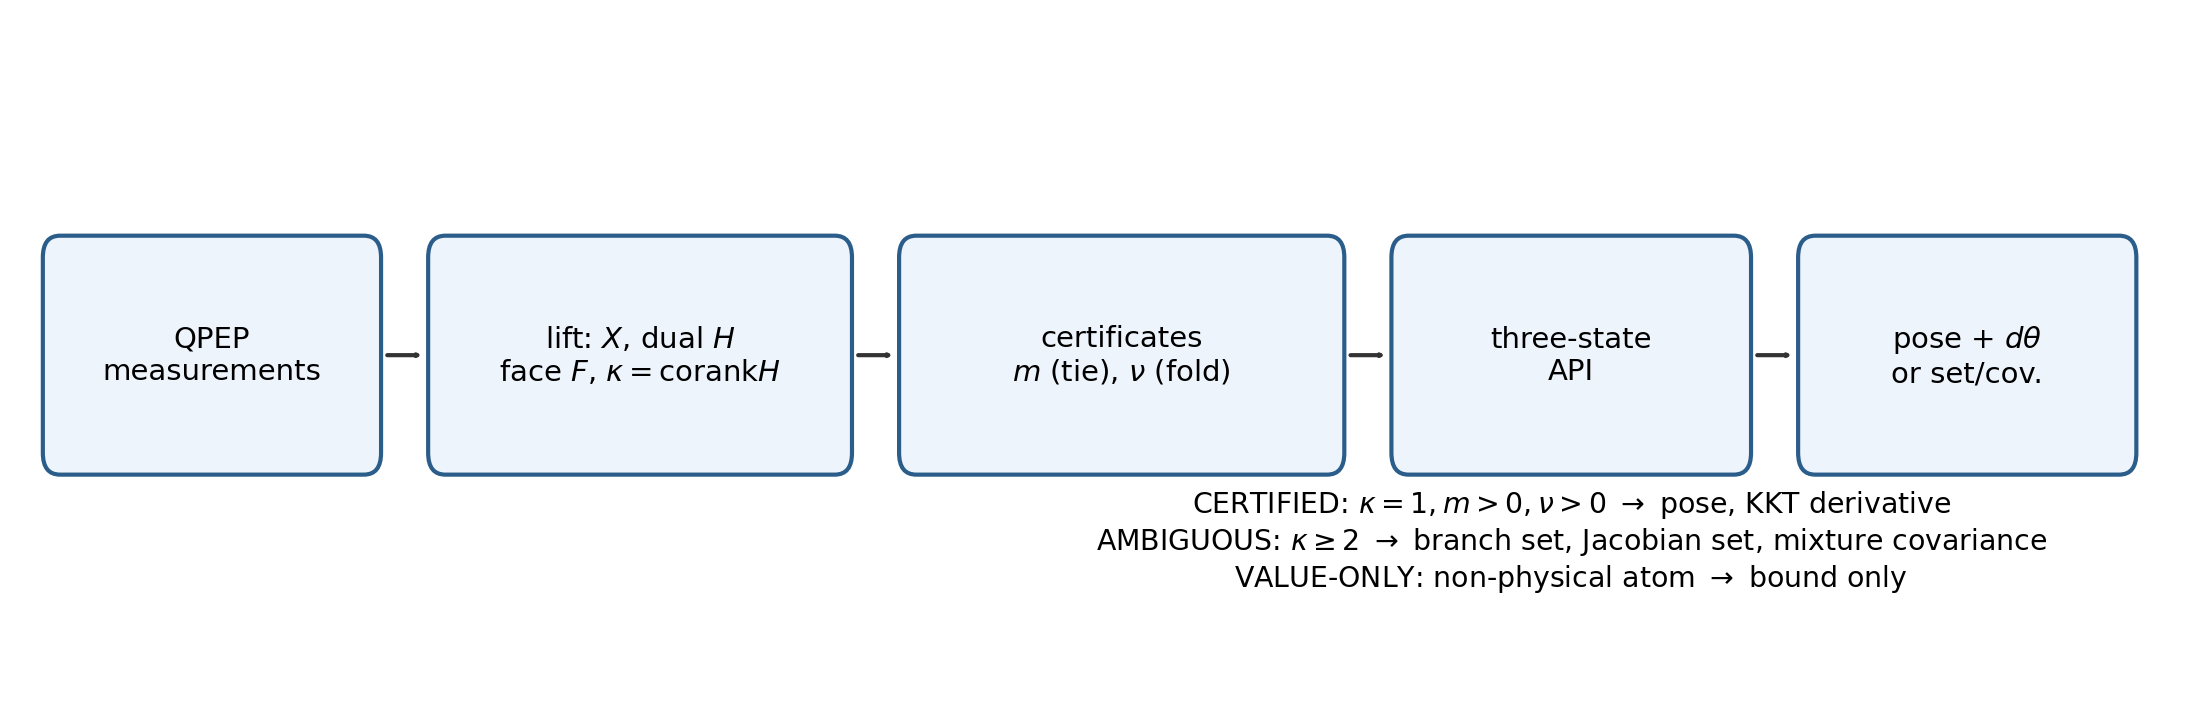
\includegraphics[width=0.9\textwidth]{figures/fig_fcd.png}
\caption{Atomic Pose Layers. The lifted SDP exposes an optimal face; a dual certificate exposes the face rank and margins (numerically in this paper). Only a single physical atom is eligible for CERTIFIED; a multi-atomic face is AMBIGUOUS; a non-physical face is VALUE-ONLY.}
\label{fig:fcd}
\end{figure*}

\section{Experiments}
\label{sec:exp}
\paragraph{Setup.} We use synthetic PnP with $n=8$ points, noise $\{0,10^{-3},10^{-2}\}$, and a planar four-point target with an exact flip. The forward candidates are local SLSQP solves from four deterministic quaternion starts, plus four fixed random starts in the 3-point experiment; the 3D negative control uses four starts. The SDP is solved with SCS. The KKT derivatives are differentiated with respect to a signed measurement perturbation. All experiments run on CPU; code and JSON are in the supplement.

\paragraph{R-form and q-form diagnostics.} Table~\ref{tab:tax} and Table~\ref{tab:diag} summarize the corrected picture. For generic PnP the $12\times12$ lift returns a unique rank-one atom $\bX^\star=\bx\bx^\top$; the sign is the two-to-one section, resolved by $\det\bR=+1$, and the $13\times13$ homogenization's last-row section is the $\bR=0$ artifact. On noiseless q-form data the measured gap is zero up to the SCS tolerance (one seed gives $-2.5\times10^{-8}$); $\dim\ker\bW=6$--$7$ and the returned moment matrix matches that nullity up to the same tolerance, with the $10^{-3}$ numerical exception noted in Table~\ref{tab:diag}. The face, not the gap, is the diagnostic.

\begin{table}[t]
\centering
\caption{Tightness taxonomy on QPEP PnP. Only a single physical atom supports a single pose and derivative. The R-form's $\pm$ is a two-to-one section of $\bX=\bx\bx^\top$, not a second atom.}
\label{tab:tax}
\setlength{\tabcolsep}{2.6pt}
\resizebox{\columnwidth}{!}{%
\begin{tabular}{lccccc}
\toprule
setting & value-tight & rank-1 attained & rank-1 returned & unique $\bX$ & physical pose \\
\midrule
generic R-form $12\times12$ & yes & yes & yes & yes & unique ($\det\bR=+1$) \\
generic R-form $13\times13$ & yes & yes & no (last row) & no & artifact ($\bR=0$) \\
generic q-form & yes ($0$) & yes & no (interior) & no (rank 6--7) & unique up to gauge \\
planar PnP & yes ($0$) & yes & no & no & two atoms (flip) \\
\bottomrule
\end{tabular}}
\end{table}

\begin{figure}[t]
\centering
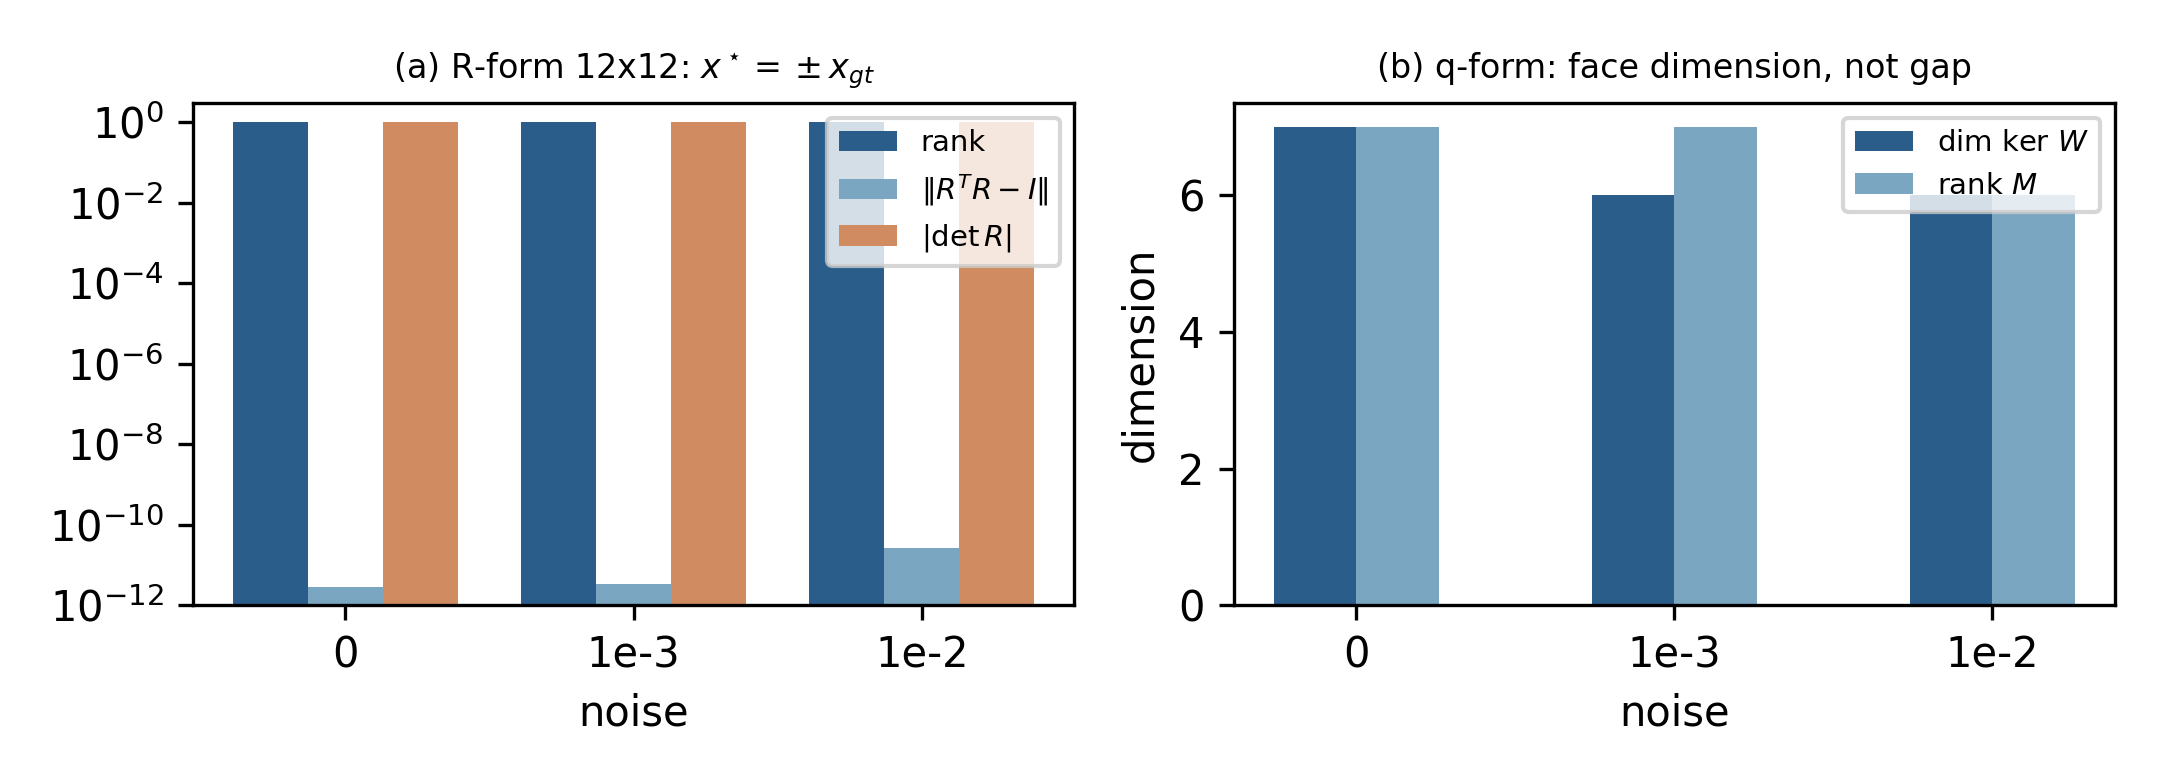
\includegraphics[width=\columnwidth]{figures/fig_face.png}
\caption{(a) The generic R-form $12\times12$ lift returns a unique rank-one atom $\bX^\star=\bx\bx^\top$; the sign is a two-to-one section resolved by $\det\bR=+1$, and the $\bR=0$ artifact is a last-row section of the $13\times13$ homogenization. (b) The noiseless q-form gap is zero up to solver tolerance; the nullity of $\bW$ is the diagnostic.}
\label{fig:face}
\end{figure}

\begin{table}[t]
\centering
\caption{Corrected diagnostics (median over 3 seeds; both ranks use the same $10^{-8}$ relative tolerance). The R-form returns a unique atom; the noiseless q-form gap is zero up to the SCS tolerance. $^\dagger$At $10^{-3}$ the numerical rank exceeds $\dim\ker\bW$ by one; the optimality residual there is at the solver tolerance, so this is a numerical rank artifact, not a counterexample to Theorem~\ref{thm:value-face} for exact optima.}
\label{tab:diag}
\setlength{\tabcolsep}{2.6pt}
\resizebox{\columnwidth}{!}{%
\begin{tabular}{lcccccc}
\toprule
noise & \multicolumn{3}{c}{R-form $12\times12$} & \multicolumn{3}{c}{q-form} \\
\cmidrule(lr){2-4}\cmidrule(lr){5-7}
 & rank & $|\det|$ & $\|\bR^\top\bR-\bI\|_F$ & $\dim\ker\bW$ & rank $\bM$ & gap \\
\midrule
$0$ & 1 & 1 & $10^{-11}$ & 7 & 7 & $0$ ($|{\rm gap}|\le2.5\times10^{-8}$) \\
$10^{-3}$ & 1 & 1 & $10^{-11}$ & 6 & $7^\dagger$ & $1.6\times10^{-5}$ \\
$10^{-2}$ & 1 & 1 & $10^{-11}$ & 6 & 6 & $2.0\times10^{-3}$ \\
\bottomrule
\end{tabular}}
\end{table}

\paragraph{Planar double cover.}\label{sec:planar} A four-point planar target has two exact poses: the true branch and its flip, with costs $1.0\times10^{-15}$ and $1.0\times10^{-15}$ and pose errors $0$ and $\pi$. The local identity solve returns the true branch; the global solver returns a set. The returned planar $\bX$ has numerical rank $4$ and the q-form nullspace has dimension $10$; the value gap is zero. The API returns AMBIGUOUS, not a pose or a derivative. Figure~\ref{fig:cover} shows the two equal-cost atoms.

\begin{figure}[t]
\centering
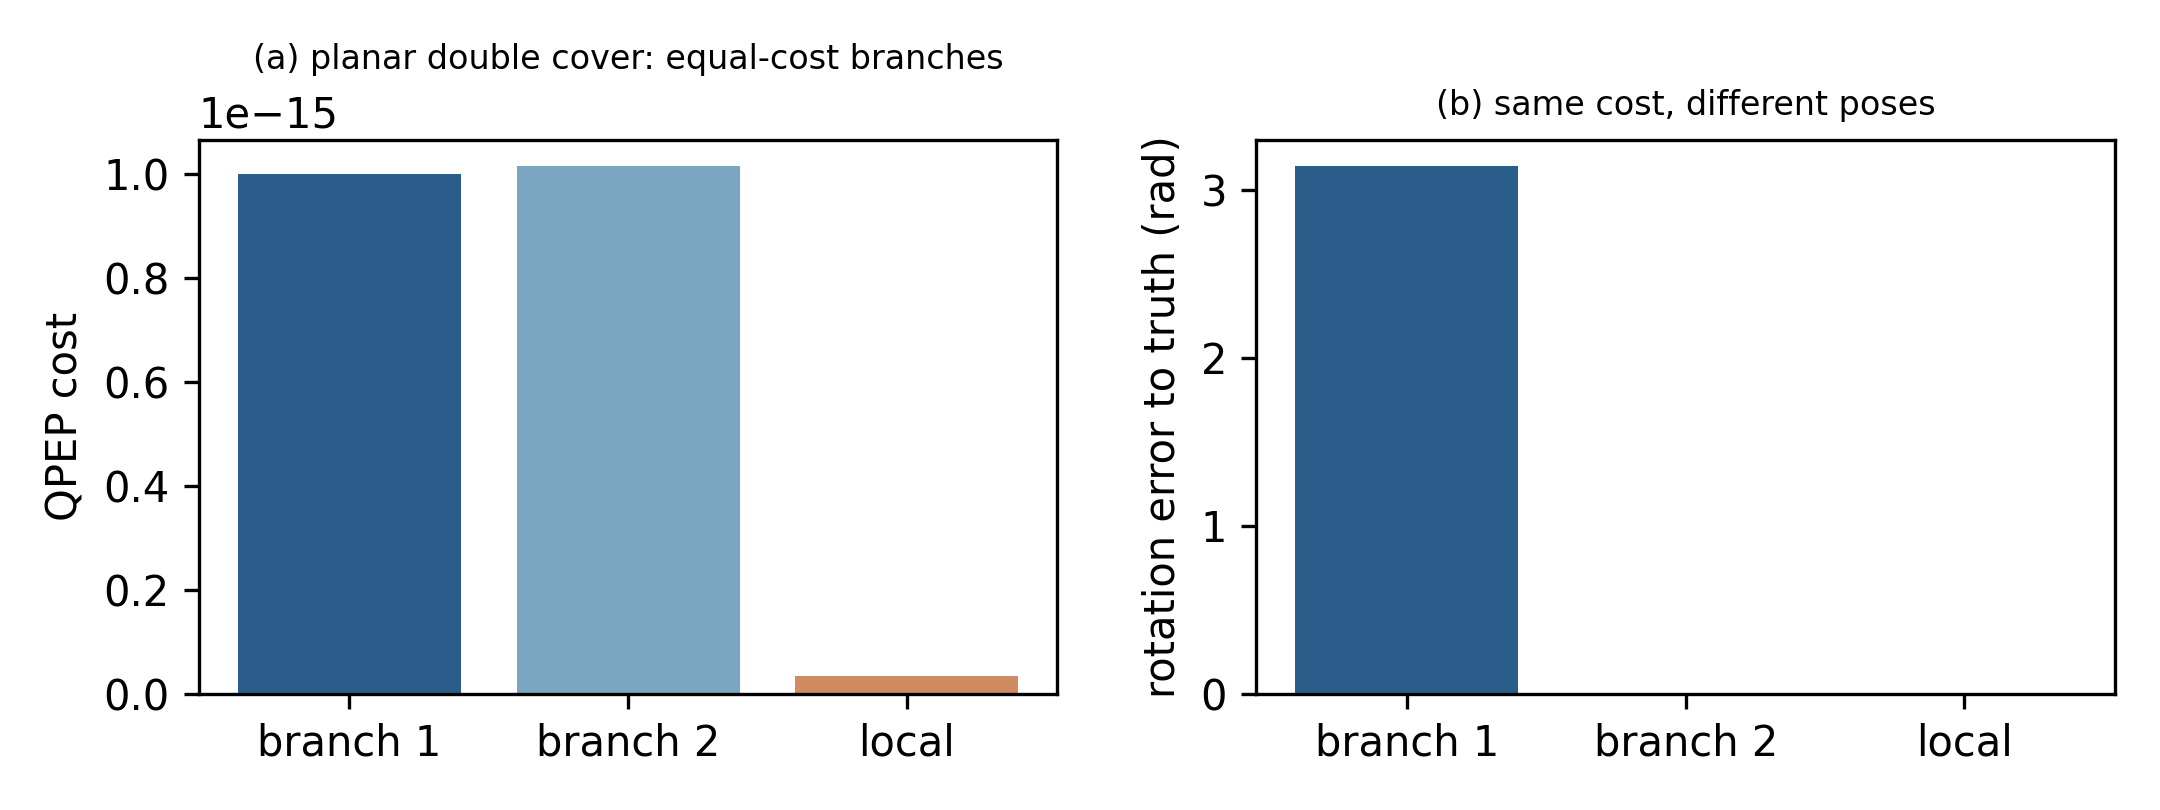
\includegraphics[width=\columnwidth]{figures/fig_double_cover.png}
\caption{Planar PnP double cover: the two branches are two distinct rank-one atoms with identical algebraic cost and poses differing by $\pi$. The face is multi-atomic; no image-only gradient can choose.}
\label{fig:cover}
\end{figure}

\paragraph{Minimal 3-point PnP (selection experiment).} We remove one of four planar points, leaving a minimal 3-point PnP. We generate $500$ instances (noise $5\times10^{-4}$) and a heading cue $\bh\sim\mathcal{N}(\bh_{\mathrm{true}},0.25^2)$, a \emph{noisy measurement of the true heading}, not the branch label. Candidates are eight QPEP starts (four deterministic, four fixed random) and OpenCV P3P (median two solutions); the cue scores a branch by $\bh(\bq)^\top\hat{\bh}$. On the QPEP set the cue raises success from $27.0\%$ (cost selection) to $80.8\%$, $+16.4$ over cue-initialized local solving ($64.4\%$). A same-start ablation gives $79.4\%$ at four starts and $80.8\%$ at eight, and cue-init with eight starts gives $79.0\%$; the gain is selection, not starts. P3P+cue reaches $86.6\%$ (oracle $98.8\%$), so the QPEP candidate set is the bottleneck: $8.8$ points are selection errors inside it ($89.6$ versus $80.8$), $10.4$ points are recall ($100$ versus $89.6$). A random-cue control drops to $28.8\%$. We do not claim SOTA; the certificate/API and KKT derivative are not exercised here.

\begin{table}[t]
\centering
\caption{Minimal 3-point planar PnP ($500$ instances, normalized image noise $5\times10^{-4}$). Success: rotation error $<0.1$ rad. The cue is a noisy measurement of the true heading ($\sigma=0.25$); the random-cue row replaces it with a random unit vector. Oracle: best branch in the generator's candidate set.}
\label{tab:cue}
\setlength{\tabcolsep}{2.4pt}
\resizebox{\columnwidth}{!}{%
\begin{tabular}{lc cc}
\toprule
method & success & median err & mean err \\
\midrule
local KKT & 0.264 & 2.968 & 2.059 \\
multi-start best-found (8) & 0.270 & 2.917 & 2.029 \\
cue-init local (1) & 0.644 & 0.0052 & 0.773 \\
cue-init local (8) & 0.790 & 0.0031 & 0.384 \\
atomic QPEP (4) & 0.794 & 0.0031 & 0.374 \\
atomic QPEP (8) & 0.808 & 0.0031 & 0.339 \\
random cue (8) & 0.288 & 2.968 & 1.958 \\
P3P + cue & 0.866 & 0.0026 & 0.172 \\
P3P oracle & 0.988 & 0.0023 & 0.013 \\
QPEP oracle (8) & 0.896 & 0.0027 & 0.163 \\
\bottomrule
\end{tabular}}
\end{table}

\paragraph{Non-planar 3D (negative control).} On a non-planar eight-point benchmark ($299$ instances, noise $10^{-3}$; with and without a $10\%$ outlier), the atomic layer is \emph{not} better. We compare local KKT; multi-start best-found (lowest cost over four starts); cue-initialized local; ``OpenCV (best of 4)'', the best of OpenCV's ITERATIVE/EPnP/SQPNP variants (an oracle over its own modes); and atomic (four starts). Multi-start best-found reaches $99.3\%$/$86.0\%$, OpenCV (best of 4) $100\%$/$89.6\%$, and atomic $96.7\%$/$84.9\%$ without/with an outlier. The cue can select a wrong branch when the algebraic cost already separates the branches; the minimal 3-point near-degenerate case is the positive case. We report this negative control to avoid overclaiming.

\paragraph{Switch and fold.} On the 1D quartic $J(x;\theta)=(x^2-1)^2+\theta x$, the branches tie at $\theta=0$; the central difference across the tie grows as $1/h$, while the one-sided branch derivative is $1/8$ (Figure~\ref{fig:switch}(b)). At the fold $|\theta|=8/(3\sqrt3)=1.5396$, the stable branch disappears and the analytic derivative $|dx^\star/d\theta|$ grows as the distance to the fold decreases; the FD/analytic ratio follows the $\nu^{-1/2}$ prediction. The tie and fold are the two failure modes of the $(m,\nu)$ certificate.

\paragraph{KKT versus finite difference.} Table~\ref{tab:kkt} compares \eqref{eq:ift} with a central difference of the same tracked branch. The median relative error is $7.4\times10^{-6}$ at $h=10^{-5}$; at $h=10^{-6}$ roundoff dominates for ill-conditioned instances (median condition number $623$). This validates the derivative on the certified stratum; it does not validate a branch that the solver did not select.

\begin{table}[t]
\centering
\caption{Relative error of the KKT derivative against a central difference of the same branch (median over 6 PnP instances).}
\label{tab:kkt}
\setlength{\tabcolsep}{3pt}
\begin{tabular}{lccc}
\toprule
$h$ & median & max & median cond$(\bK)$ \\
\midrule
$10^{-3}$ & $3.9\times10^{-4}$ & $5.6\times10^{-4}$ & 623 \\
$10^{-4}$ & $3.9\times10^{-5}$ & $5.6\times10^{-5}$ & 623 \\
$10^{-5}$ & $7.4\times10^{-6}$ & $3.5\times10^{-4}$ & 623 \\
$10^{-6}$ & $8.8\times10^{-4}$ & $3.2\times10^{-2}$ & 623 \\
\bottomrule
\end{tabular}
\end{table}

\paragraph{Uncertainty.} On a synthetic two-mode posterior the single-branch Laplace variance is $0.030$ while the posterior variance is $0.805$ (a $27\times$ underestimate); the Laplace-mixture variance is $0.898$ (the exact posterior is $0.805$). A one-step risk-sensitive action under the mixture costs $0.85$, while the single-mode action costs $2.77$ under the true mixture. We report this as a synthetic illustration of \eqref{eq:cov}, not as a 3D robot result.

\begin{figure}[t]
\centering
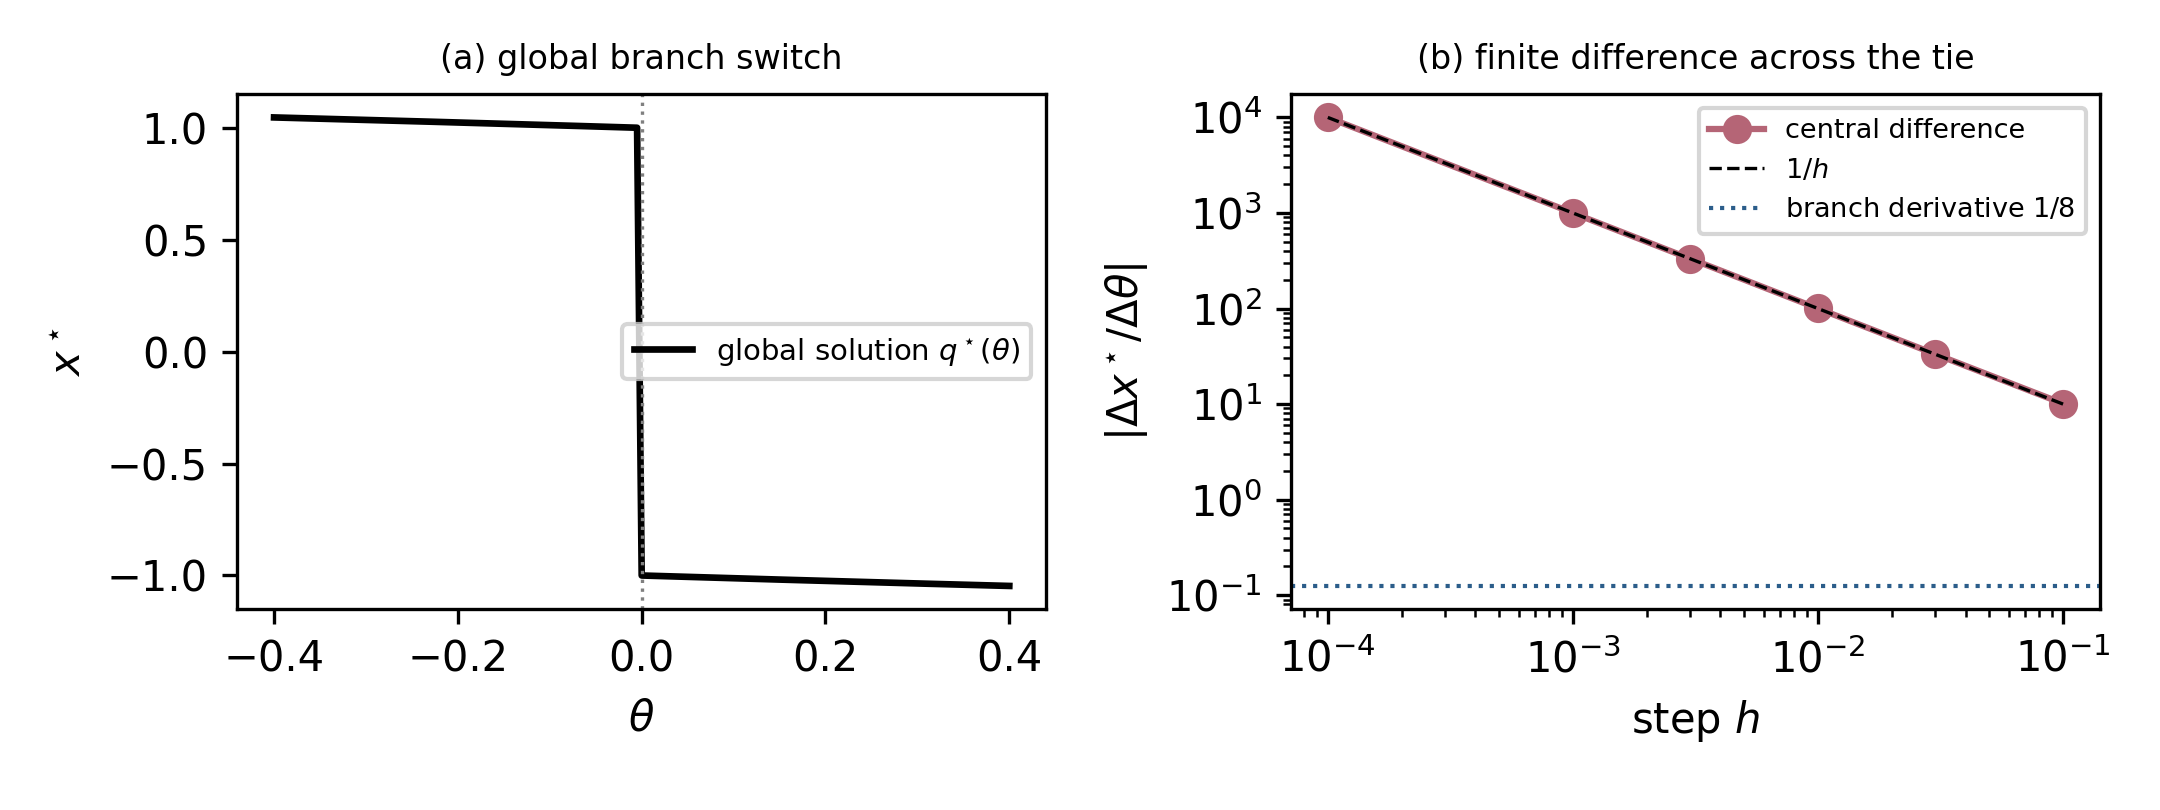
\includegraphics[width=0.92\columnwidth]{figures/fig_switch.png}
\caption{(a) Global solution switches at the tie. (b) Central difference across the tie diverges as $1/h$; the one-sided branch derivative is $1/8$.}
\label{fig:switch}
\end{figure}

\begin{figure}[t]
\centering
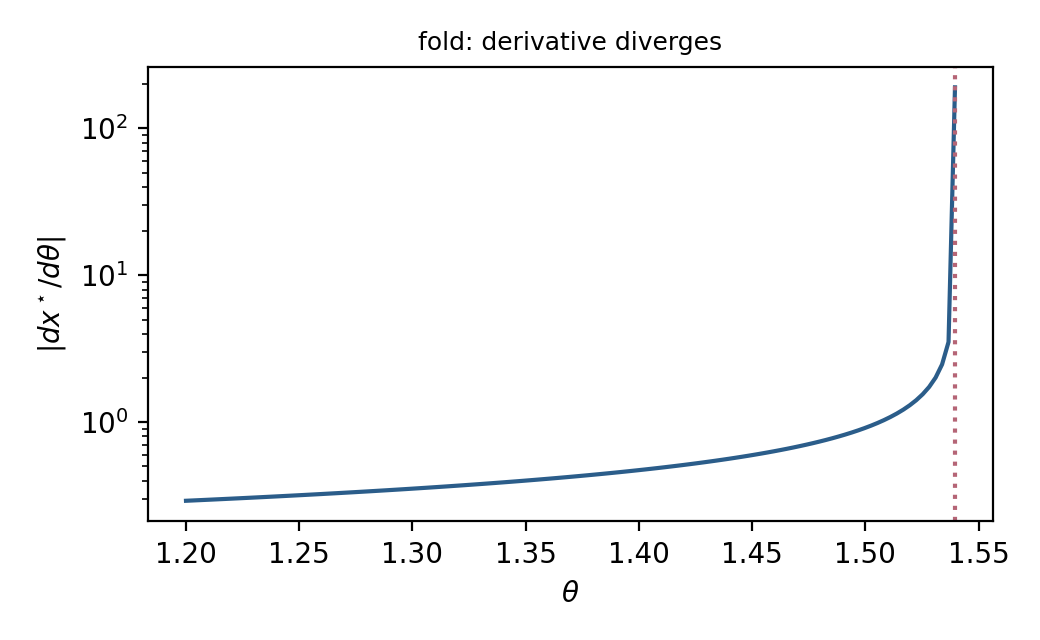
\includegraphics[width=0.92\columnwidth]{figures/fig_fold.png}
\caption{At the fold $|\theta|=1.5396$ the disappearing branch's derivative diverges; this is the $\nu^{-1/2}$ failure mode, distinct from the tie discontinuity.}
\label{fig:fold}
\end{figure}

\section{Discussion and Limitations}
FCD changes the contract, not the solver: a layer should report its face and margins, and emit a pose and derivative only for a single physical atom. The experiments support: the R-form is tight with a unique atom and a two-to-one section; the planar face has two atoms; the noiseless q-form gap is zero up to solver tolerance; the KKT derivative is correct on the certified stratum and fails at ties/folds. The 3-point experiment validates selection, not the certificate/API: no three-state certificate or KKT derivative is run, only rotation success is scored, and the forward is an eight-start heuristic. P3P+cue is stronger ($86.6\%$ versus $80.8\%$), so the QPEP candidate set is the bottleneck. The SCS dual is numerical, not strict: over $20$ seeds, median minimum eigenvalue $-1.6\times10^{-7}$ (worst $-8.8\times10^{-5}$) and median $\tr(\bH\bX)=3.9\times10^{-6}$ (worst $1.45\times10^{-5}$), with one rank-5 seed; $\corank\bH$ and state counts are not computed, so we do not claim a verified certificate. The covariance experiment is 1D synthetic; no 3D end-to-end result is claimed.

\section{Conclusion}
Differentiability of a global estimator is a property of its face, not its value. QPEP's R-form has a unique atom and a two-to-one section, planar PnP two equal-cost atoms, and its quaternion gap is zero. FCD certifies a derivative only on the unique physical stratum and refuses a silent gradient when the face is ambiguous. On the minimal 3-point benchmark, cue-conditioned selection reaches $80.8\%$ ($64.4\%$ for cue-init) and P3P+cue $86.6\%$, locating the gap in the QPEP candidate set.

\bibliographystyle{IEEEtran}
\bibliography{references}
\end{document}
